%%=============================================================================
%% Interview Sadith
%%=============================================================================

\chapter{Interview met Sadith, Añañau}
\label{ch:interviewSadith}

%% TODO: Hoe ben je te werk gegaan? Verdeel je onderzoek in grote fasen, en
%% licht in elke fase toe welke stappen je gevolgd hebt. Verantwoord waarom je
%% op deze manier te werk gegaan bent. Je moet kunnen aantonen dat je de best
%% mogelijke manier toegepast hebt om een antwoord te vinden op de
%% onderzoeksvraag.
\section{Inleiding}
Om een antwoord te kunnen bieden op de eerst onderzoeksvraag, werd ervoor gekozen om een interview af te nemen van Sadith Paez Montesinos. Sadith is één van de mede-oprichtsters van Añañau. Zij staat vandaag in voor de dagdagelijkse werking (het administratieve, educatieve, financiele luik). Ze stuurt, samen met Ellen Bosch, een 10 tal medewerkers en vrijwilligers aan. Añañau is een non-profit en niet-gouvernementele organisatie die in december 2014 werd opgericht in Cusco, Peru. De organisatie werkt met kinderen en jongeren tussen 4 en 18 jaar oud die in situaties van extreme armoede en onstabiele familiesituaties leven in het district San Jeronimo, een buitenwijk van Cusco. Sinds januari 2015 is de organisatie als officiële NGO erkend in Peru. Omdat ze geloven in de kracht van goed en inclusief onderwijs als springplank naar een betere toekomst, is Añañau in de eerste plaats een educatief project. Via huiswerkbegeleiding en spelend leren stimuleert Añañau de ontwikkeling van de kinderen en tracht ze nieuwe kansen te creëren. \autocite{Ananau2020}

Door haar ervaring in het werkveld beschikt Sadith over relevante informatie omtrent het onderwijs in Peru, die interessant kan zijn voor dit onderzoek. Dit interview werd, door de huidige maatregelen tegen het Covid-19 virus, afgenomen vanop afstand.

In Figuur \ref{sadith} is Sadith te zien.

 \begin{figure}[h!]
	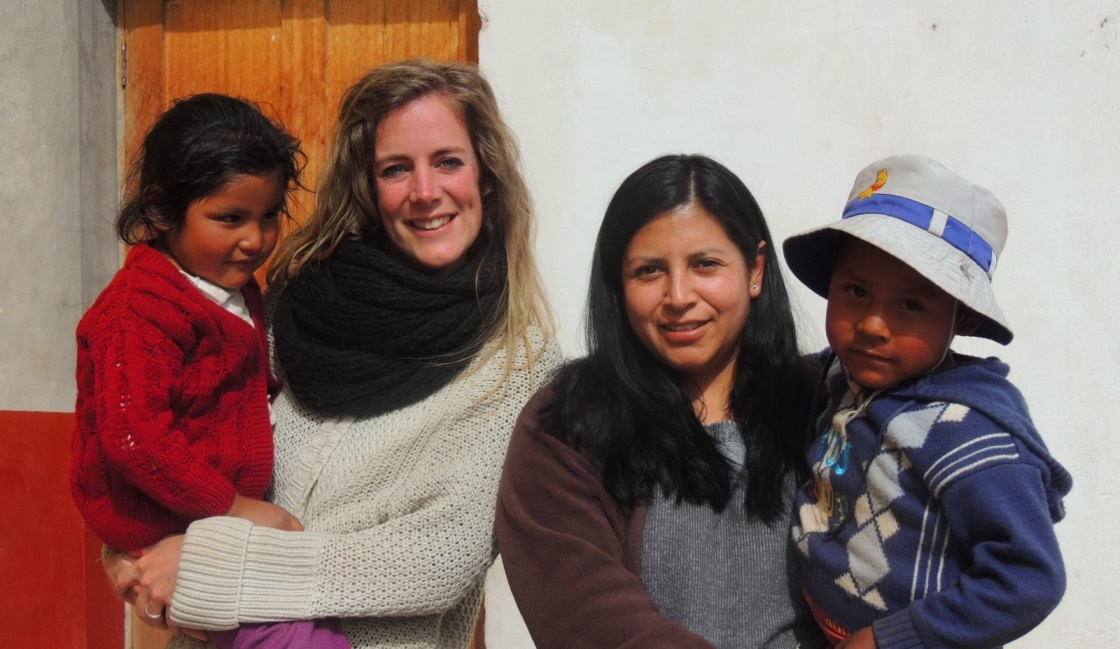
\includegraphics[width=\textwidth]{../img/sadith.jpeg}
	\caption{Oprichtsters Añañau: Links Ellen Bosch, Rechts Sadith Paez Montesinos} \autocite{Ananau2020}
	\label{sadith}
\end{figure}

\section{Interview}
\textbf{Hebben de meeste staatsscholen in Peru computers ter beschikking op school? Welke apparatuur wordt er gebruikt? Zijn er problemen met deze apparatuur?}

\textit{Sadith:} Niet alle scholen hebben computers. Van de scholen die zich in de binnenstad bevinden heeft volgens mij 80\% van de scholen één of meerdere computers ter beschikking. Bij de scholen buiten de stad, in het binnenland van Peru dus, is dat volgens mij slechts 40\% van de scholen. Als een school computers heeft, zijn dat er ongeveer 10 of 20 computers per 200 à 220 leerlingen.

\textbf{Hoe gebruiken de kinderen de computers op school om te leren?}

\textit{Sadith:} Normaal gezien gebruiken ze de computers om informaticalessen te krijgen. De leerlingen gaan dus niet voor andere vakken aan de slag met informatica. 

\textbf{Wat leren de kinderen dan tijdens de computerlessen?}

\textit{Sadith:} Ze leren specifieke programma's gebruiken. Ze leren niet programmeren, maar leren vooral praktisch werken met bijvoorbeeld Microsoft Word en Microsoft Excel.

\textbf{Passen de staatsscholen informatica binnen hun curriculum nog op andere manieren toe, zoals met het gebruik van smartboads of tablets?}

\textit{Sadith:} Smartboads hebben de scholen niet. Ongeveer 5 jaar geleden werd een project opgestart waarbij het gebruik van tablets op scholen gestimuleerd werd. Dit lukte in de grote steden van Peru, maar in het binnenland was er meestal geen internetverbinding. Hier in Peru moeten we elke 5 jaar gaan stemmen en verandert de samenstelling van de regering. Het komt vaak voor dat nieuwe regeringen een andere aanpak hebben, en niet meer in de bestaande projecten willen investeren. Na de laatste regeringswissel werd het tablet project stopgezet.

Nu sinds kort, zitten we in de huidige covid-19 crisis. Daardoor investeert de overheid op dit moment in ICT projecten voor het onderwijs, omdat alle leerlingen thuis moeten blijven, en er studeren. Onlangs kochten ze nog 13.000 computers aan die via satellieten kunnen verbinden met het internet. Deze computers zouden dienen om aan studenten uit te delen, zodat ze thuis op de computer voor school kunnen werken. 

\textbf{Moeten kinderen die naar staatsscholen gaan soms huiswerk maken op computers? Wat moeten ze doen als ze geen computer hebben?}

\textit{Sadith:} Ja, de kinderen moeten thuis huiswerk maken op computer. Als ze thuis geen computer hebben, gaan ze naar een internetcafé. Daar kunnen ze computers gebruiken voor 1 sol per uur (ongeveer 0,25 eurocent) en printen. Hier in Peru zijn er veel internetcafés. Een nadeel is wel dat de kinderen er vaak in aanraking komen met videospelletjes. Ze worden verleid, zijn vaak afgeleid en komen niet aan huiswerk maken toe. 

\textbf{Zijn de leerkrachten voldoende opgeleid om computers te gebruiken?}

\textit{Sadith:} Niet alle leerkrachten kunnen met computers werken. Dit is een groot probleem hier. Er zijn leerkrachten die al veel ervaring hebben in het onderwijs, maar bijna op pensioen gaan. Deze 'oude generatie' leerkrachten heeft veel minder voeling met de nieuwe technologieën.

\textbf{Zijn er dan geen bijscholingen voor die leerkrachten?}

\textit{Sadith:} Op vlak van informatica moeten leerkrachten vaak zichzelf bijscholen. Dit wordt niet georganiseerd door de overheid. Er wordt dus verwacht dat de leerkrachten zelf op zoek gaan, en ervoor zorgen dat ze zelf op de hoogte zijn. In realiteit loop dit vaak fout en zijn er leerkrachten waarbij de computerkennis heel erg beperkt is. Wel bestaan er platformen die lessen aanbieden. Die lessen zijn voor alle inwoners, en niet specifiek gericht op lesgevers.

\textbf{Zijn er ICT-leerkrachten, en zijn ze opgeleid?}

\textit{Sadith:} Hier in Cusco kan je niet studeren voor ICT leerkracht. Daardoor zijn er hier niet veel opgeleide ICT leerkrachten. Enerzijds worden er vaak leerkrachten aangesteld als ICT leerkracht zonder daartoe de opleiding te hebben gekregen. Anderzijds gebeurt het soms ook dat er ICT specialisten ingezet worden. Deze specialisten zijn heel erg duur en dus vaak onbetaalbaar voor staatsscholen. Meestal geven zij de voorkeur aan een job buiten het onderwijs omdat ze elders meer kunnen verdienen. 

\textbf{Is er programmatuur die kan gebruikt worden op de computers door de kinderen, zoals een taal- of rekenprogramma?}

\textit{Sadith:} Ja, er bestaan educatieve computers die specifiek ontworpen zijn om te gebruiken in de les of voor huiswerk. Op die computers staan de nodige programmatuur, ook al hoor ik vaak dat die erg verouderd is.
	
\textbf{Zijn er digitale omgevingen waarop kinderen kunnen aanloggen?}

\textit{Sadith:} Vroeger niet, maar recent (sinds een maand) is de overheid begonnen met het ontwikkelen van een platform. Door de recente uitbraak van het covid-19 virus voorziet de overheid een platform waarop kinderen van thuis uit kunnen les volgen. Het platform heet 'Aprendo en casa' (vertaald: ik leer thuis, https://aprendoencasa.pe/). Natuurlijk bereikt het platform alleen kinderen die toegang hebben tot een computer met internetverbinding. Verder zendt de overheid ook lessen uit op de radio- en televisie. Elke leeftijdsgroep heeft een tijdsspanne waarop ze dagelijks lessen kunnen volgen. Een specifiek platform voor elke school, waarop de leerlingen kunnen inloggen bestaat naar mijn weten niet. 

Op dit moment, omwille van de pandemie, proberen leerkrachten vooral contact te houden met hun leerlingen via WhatsApp-groepen.

\textbf{Wat zijn de knelpunten op het vlak van informatica in het onderwijs in Peru? Hoe kunnen deze knelpunten weggewerkt worden?}

\textit{Sadith:} Volgens mij zijn er drie grote problemen: eerst en vooral was educatie nooit een prioriteit voor de verschillende regeringen in het verleden. Wanneer er nieuwe scholen werden gebouwd, was er meestal geen budget meer vrij om computers aan te schaffen. Er werd geïnvesteerd in gebouwen, en onvoldoende in IT materiaal. Volgens mij is geld dus de hoofdreden. Verder is vooral de infrastructuur een groot probleem. Vele scholen buiten de stad hebben geen internet-aansluiting, vaak door de moeilijke ligging, en de bergachtige geografie van Peru. Door de bergen is het vaak heel gecompliceerd, en moeten particulieren zelf antennes aanschaffen om een internetverbinding tot stand te brengen. Voor scholen zijn er dus veel kosten, en daar hebben ze meestal geen geld voor. Computers zijn vaak niet meer functioneel. De huidige regering doet zijn best om ICT bij kinderen op scholen te ondersteunen. Zoals ik al zei kochten ze zeer recent grote aantallen computers voor kinderen die geen toegang hebben tot informatica.

Het tweede probleem is, zoals ik al zei, dat telkens als de regering wijzigt er een ander plan van aanpak is. Soms zijn er heel goede projecten die bij een regeringswissel gestopt worden. Zo kan een regering dus 5 jaar lang een project opzetten en kan de volgende regering opteren dat niet meer te doen, waardoor er dus geen continuïteit is.

Het laatste probleem is dat er weinig informatica leerkrachten zijn, zoals ik eerder uitlegde. Er is hier in Cusco geen opleiding, en specialisten zijn erg duur.

Een oplossing zou kunnen zijn om, zoals wij doen op het project Añañau, krachten van mensen te bundelen en samen te zoeken naar budgetten waarmee er doelen kunnen bereikt worden. 

\textbf{Hoe komt het dat Peru niet verder staat op vlak van informatica, wat liep er fout in het verleden?}

\textit{Sadith:} Vaak is corruptie een probleem geweest in het verleden volgens mij. De huidige regering geeft duidelijk geprioriteerd aan de aankoop van computers voor scholen maar vroeger was dat niet het geval. Regeringen probeerden vaak geld in eigen zak te steken, en dat liep helemaal fout. 
 
\subsection{Conclusie}
Sadith haalde tijdens het gesprek aan dat de overheid recentelijk vele computers aankocht die verbinding maken met een satelliet om verbinding met het internet te realiseren. Op 18 april verspreidde het ministerie van onderwijs een persbericht waarin werd medegedeeld dat er 840.000 tablets worden aangekocht met mobiel internet voor schoolkinderen in afgelegen landelijke en stedelijke gebieden, zodat ze de kinderen kunnen blijven studeren en de digitale kloof kan worden verkleind. Op deze manier kunnen de kinderen onderwijs vanop afstand volgen.\autocite{Minedu2020} Nadat ik Sadith het persbericht liet lezen zei ze dat ze het inderdaad over dit bericht had in het interview. Echter werd dit tot op heden nog niet uitgevoerd. 

Ook vertelde Sadith over 'Aprendo en casa'. Dat is een programma dat de regering aanbiedt om de schoolgaande kinderen te voorzien van thuis onderwijs. Door de recente uitbraak van het covid-19 virus volgen er 6 miljoen scholieren van openbare scholen les via computer, radio en televisie. De Peruviaanse regering zorgde hiervoor. \autocite{Minedu2020a}

%Studeren in cusco voor ict leerkracht ??
